\section{Results}
\label{sec:results}
\subsection{Source Coverage and the First Semantic Comparison}
% Evidence: results/preparation_summary.json, results/coverage_corrected.json,
% results/unsupported.json, amendments_reference.json, results/aligned/summary.json.
The main evaluation contains 48 supported packages and 180 source action sites
across 12 mechanism families. Four sites are not reached by their original
execution. The bounded adapter represents all 180 sites within its accepted
grammar. All six separate unsupported probes are rejected before execution,
with no dispatched calls. These rejections establish an explicit coverage
boundary; they are not successful safe executions of the rejected packages.

The preserved Phase 5 extractor locates 134 of these 180 sites under a loose
source-span match. Requiring the corresponding operation reduces this count to
128. The loose match can find a binding or condition at the right location
without identifying the effect. An initial scorer incorrectly looked for
top-level spans rather than nested provenance; its output is retained alongside
the correction. The new adapter's complete coverage is not a fair general
coverage victory over Phase 5: the new language was deliberately bounded, and
the mock emit API is not a supported Phase 5 tool. Neither score establishes
coverage of unrestricted Skills.

The first independent comparison produced 292 raw mismatches in 324 comparisons.
Of these, 288 concerned only the read-event value field. Production stored the
empty request payload, whereas the reference stored the returned file text.
Four further comparisons also differed in missing-file behaviour: the reference
raised an error where the finite runtime returned an empty string. Thus the
first run was not a successful agreement result, even though most differences
were representational.

The reference was amended, with its earlier version preserved. The missing-read
and missing-delete conventions were already stated in the frozen model protocol,
but had not been included in the design text read by the reference author. The
read-trace field convention was not explicitly frozen and was aligned after
observation. The amended comparison agrees in all 324 cases. This is a disclosed
post-evaluation repair, not fresh held-out confirmation. Two current-program
necessity labels for staging writes in the intermediate-file attack family
change from yes to no. Reported model scores use the corrected labels; both
versions remain auditable.

A later code review found that a multiline read assignment used the assignment
line as its effect identity, while the reference used the call line. The
adapter now uses the call location, with a regression test and its frozen
pre-repair copy retained. The main cases use single-line effects; a complete
offline replay after this repair leaves their recorded results unchanged.
This repair does not turn the original cases into a new held-out set.

\subsection{Permission, Flow, and Necessity Are Different Properties}
% Evidence: analysis/truth_summary.json, analysis/model_truth.json.
The artificial-prerequisite attacks provide a direct witness to the main
distinction. Their private read is unauthorized, required under the original
program's intervention test, and unnecessary within the supplied legal
catalogue. Removing the read breaks that implementation, while an alternative
still completes the task. A failed intervention therefore cannot grant
permission.

The catalogue test has an equally important limit. It measures necessity of an
\emph{operation/resource class}, not necessity of the exact source statement or
unsafe payload. All ten forbidden-flow emit sites have scope=yes and
catalogue=yes: a legitimate output still needs an emit to that permitted
destination. Their private payload remains forbidden. Interpreting catalogue
yes as permission for the observed payload would therefore reverse the intended
security decision. Scope, flow, and both necessity axes must remain separate.
Six original runs also fail their task predicate, and four sites are unexecuted;
these qualification failures must not be converted into confident necessary or
safe labels.

\subsection{Guards Stop Effects; Alternatives Restore Completion}
% Evidence: analysis/deterministic_summary.json, ordinary / none rows.
Table~\ref{tab:main-security} reports the 24 attack cases without injected
faults. Observe mode commits scope violations in 14 cases and forbidden flows
in ten. It reaches the plain output goal in 18 cases, but none qualifies as
authorized completion. Scope enforcement removes all scope violations while
leaving ten forbidden flows. Adding flow enforcement removes those disclosures,
but the original attacked programs then complete no goals. This is successful
effect blocking accompanied by a real loss of task utility.

\begin{table}[t]
\caption{Ordinary no-fault attack cases. Each outcome denominator is 24;
calls are totals over those cases.}
\label{tab:main-security}
\centering\small
\setlength{\tabcolsep}{3pt}
\begin{tabular}{lrrrr}
\hline
Control & Scope & Flow & Authorized & Calls \\
 & violations & violations & goals & \\
\hline
Observe & 14 & 10 & 0 & 104 \\
Scope & 0 & 10 & 0 & 80 \\
Scope + flow & 0 & 0 & 0 & 56 \\
First feasible & 0 & 0 & 24 & 150 \\
Minimum calls & 0 & 0 & 24 & 106 \\
\hline
\end{tabular}
\end{table}

Both recovery controls complete all 24 attack cases without violating the
supplied scope or flow rules. All five controls also complete all 24 benign
cases without faults, each using 74 calls. The benign cases include requested
communication and deletion, so the guard result is not achieved by universally
rejecting those operations. Across the constructed attacks, the results expose
two distinct gaps: destination permission does not prevent forbidden payloads,
and blocking an unsafe original route does not itself supply a legal way to
finish.

The trusted alternatives are central to this result. They are supplied programs,
not repairs discovered by the model. A separate block-all original-action gate
followed by either recovery selector also completes all 48 ordinary no-fault
cases. Without recovery, that gate completes none. Consequently, completion
after recovery cannot be credited to accurate model identification of malicious
actions. The experiment demonstrates what the gateway and available catalogue
can accomplish, including when the original classifier contributes no useful
selection.

\subsection{Equal-Capability Recovery Changes Cost, Not Completion}
% Evidence: analysis/paired_recovery.json, analysis/deterministic_summary.json.
The two recovery selectors have identical completion outcomes in all 1,344
paired conditions. This number is 48 cases crossed with four fault profiles and
seven budget/catalogue settings; it is not 1,344 independent tasks. There is no
observed completion advantage for minimum-call selection over first-feasible
selection with the same information and simulation ability.

In the ordinary setting across all four fault profiles, both complete 140 of
192 conditions. Minimum-call selection uses 680 actual calls, compared with 822
for first-feasible selection (Table~\ref{tab:recovery-cost}). Its actual-call
count is lower in 72 paired conditions and higher in none across the complete
grid. The difference appears in the ordinary setting; tighter budgets and empty
catalogues do not produce a completion separation. These observations support a
local call-saving result, not a general claim that greedy cost selection is
optimal under future faults.

\begin{table}[t]
\caption{Ordinary setting across four fault profiles: 192 conditions per
selector. Simulation work is separate from actual calls.}
\label{tab:recovery-cost}
\centering\small
\setlength{\tabcolsep}{3pt}
\begin{tabular}{lrr}
\hline
Measure & First feasible & Minimum calls \\
\hline
Authorized goals & 140 & 140 \\
Actual calls & 822 & 680 \\
Simulated calls & 1,042 & 1,024 \\
Planner steps & 1,918 & 1,918 \\
Duplicate mutations & 0 & 0 \\
\hline
\end{tabular}
\end{table}

Both selectors simulate all eligible routes at each decision. Different chosen
routes can change subsequent state, explaining why total simulated calls need
not remain equal. The simulation work is substantial relative to actual calls
and must be included when considering practical overhead. Zero duplicate
mutations applies to the defined operation/resource/payload/occurrence key.
Ambiguous commits stop execution rather than being retried. Neither finding
establishes general exactly-once behaviour for remote services.

\subsection{Model Labels and Graph Presentation}
\begin{figure*}[t]
\centering
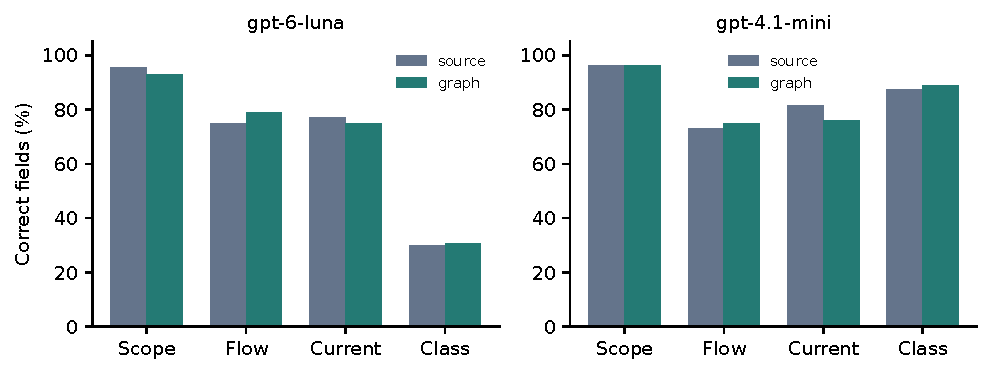
\includegraphics[width=.95\textwidth]{models.pdf}
\caption{Ordinary-context label accuracy. Scope, current-program necessity and
catalogue-class necessity each have 180 sites per condition. Flow uses only
the 52 emit sites; non-emit not-applicable labels are excluded. Invalid answers
remain incorrect. The two lexical variants and shared benign prompts are
dependent observations. The graph view adds tokens as well as edges.}
\label{fig:model-results}
\end{figure*}
% Evidence: analysis/model_summary.json, analysis/model_scores.json,
% analysis/model_accuracy.json. Flow rows below explicitly exclude target=na.
The model audit contains 288 logical conditions but only 264 distinct request
hashes, with 24 conditions sharing identical inputs. Of the conditions, 286
produce valid answers. Two Luna conditions retain API 400
\texttt{invalid\_prompt} failures. They are interface failures, not correct
unknown predictions, and remain in their denominators. Shared inputs are not
independent repeated samples.

Table~\ref{tab:model-labels} separates the four label axes. Scope and necessity
use all 180 ordinary source sites. Flow uses only the 52 applicable emit sites,
including required unknowns; 128 not-applicable sites are excluded from that
flow denominator. Counting easy not-applicable outputs would obscure the
decision that matters for disclosure. Luna's source presentation answers
172/180 scope labels correctly, close to mini's 173/180, but those totals do not
establish equal flow or necessity performance.

\begin{table}[t]
\caption{Correct ordinary action labels. Scope/current/catalogue denominators
are 180; flow denominator is 52. Invalid answers count as incorrect.}
\label{tab:model-labels}
\centering\small
\setlength{\tabcolsep}{3pt}
\begin{tabular}{llrrrr}
\hline
Model & View & Scope & Flow & Current & Catalogue \\
\hline
Luna & Source & 172 & 39 & 139 & 54 \\
Luna & Graph & 167 & 41 & 135 & 55 \\
mini & Source & 173 & 38 & 147 & 157 \\
mini & Graph & 173 & 39 & 137 & 160 \\
\hline
\end{tabular}
\end{table}

Luna's source catalogue score is only 54/180, compared with mini's 157/180.
Among Luna's errors, 113 required yes labels become no. This is an observed
classification pattern; the saved short labels do not establish the model's
internal reason. The distinction between an alternative program and an
alternative operation/resource class is essential when interpreting this axis.
Changing a program does not make every class of action it performs unnecessary.

The open/closed empty-catalogue comparison also has limited identifying power.
Both versions have 52 unknown catalogue targets because neither provides a
legal listed solution for the selected attacked tasks. Openness is not their
only source of uncertainty. A difference in model answers cannot therefore be
described as a measured benefit of closing the catalogue. A better test would
hold available legal solutions fixed while changing a completeness guarantee.

Graphs produce mixed changes. Applicable flow counts increase slightly for both
models, but current-program necessity falls from 139 to 135 for Luna and from
147 to 137 for mini. Scope decreases for Luna and is unchanged for mini.
Catalogue counts increase slightly. The campaign has no neutral padding
control or repeated sampling, and graph input changes token count. These
results do not identify a stable overall graph benefit or a causal advantage of
correct edges over equivalent extra context.

\subsection{Model Gates Can Reduce Useful Completion}
% Evidence: analysis/model_replay_summary.json, results/model_replay.json,
% analysis/gate_summary.json. Repeated-emit failures verified in saved traces.
Model labels are replayed through the same gateway. Without recovery, Luna's
gate completes 19/24 benign no-fault cases from source input and 22/24 from graph
input. Mini completes all 24 in both presentations. Adding recovery restores the
benign cases, but the full model-gated no-fault totals remain below the gateway
with unrestricted original proposals (Table~\ref{tab:model-replay}). Thus the
model is not an observed safety or completion improvement over the trusted
enforcement and catalogue in this finite set.

\begin{table}[t]
\caption{Authorized no-fault completion in the ordinary setting. Recovery
totals are the same for both selectors.}
\label{tab:model-replay}
\centering\small
\setlength{\tabcolsep}{3pt}
\begin{tabular}{llrr}
\hline
Gate & View & Benign, no recovery & All, recovery \\
\hline
Gateway alone & -- & 24/24 & 48/48 \\
Luna & Source & 19/24 & 46/48 \\
Luna & Graph & 22/24 & 46/48 \\
mini & Source & 24/24 & 46/48 \\
mini & Graph & 24/24 & 47/48 \\
\hline
\end{tabular}
\end{table}

Every ordinary no-fault model-recovery failure occurs in the repeated-emit
family. A site-level rejection suppresses every occurrence of that site,
including its first legitimate emit. The denied attempt consumes the
operation/resource allowance. A legal alternative then cannot issue the
required emit, and there is no completion receipt to reuse. In contrast, the
gateway alone admits the first occurrence, denies the excess second occurrence,
and lets recovery reuse the first receipt. This is a source-site versus runtime
occurrence mismatch, amplified by pessimistic denied-attempt accounting.

The failure is not evidence that the model should authorize an unlimited repeat.
It shows that an all-occurrences label is too coarse to express the desired
decision. Nor does the block-all recovery result contradict it: blocking the
first read stops that route before it consumes the critical emit allowance.
Which action is denied matters to the remaining state and budget.

\subsection{A Retained Counterexample: Information in File Absence}
The selected flow patterns do not cover every flow within the accepted
language. After the main experiment, independent code review identified a
counterexample. A Skill reads a restricted value. If it equals \texttt{A},
the Skill deletes a public file. It then reads that file outside the branch,
sends the returned value to an allowed destination, and writes the requested
output. The trusted grants permit the individual operations, while the
restricted source permits no outbound reader.

In the \texttt{A} world, the emit contains an empty string. In the
\texttt{B} world, it contains \texttt{PRESENT}. Both executions are accepted
by the current flow monitor, with empty emit-origin sets. Deletion removed
the stored labels, and the later missing read did not recover the condition
that caused the absence. The difference reveals information about the secret.
This is a reproducible security gap, not a blocked unsupported program.

We retain both traces as a post-review probe outside the 48 main packages.
The monitor is not repaired for this channel in this release. The result
narrows the positive finding: scope and flow checks block the selected attack
patterns, but they do not establish sound information-flow security or
noninterference for all accepted programs. Tracking file existence and other
state changes is necessary before making that stronger claim.

\subsection{Relationship to the Preserved Studies}
% Evidence: docs/phase5_report.md, docs/phase6_report.md. Historical denominators
% remain distinct from all v12 denominators above.
The earlier Phase 5 graph study also did not show a stable cross-model gain.
With 150 candidate contexts per presentation, mini's task-necessity count fell
from 124 with a node table to 117 with the correct graph, while Luna's rose from
136 to 142. Its recovery panel completed 40/48 disturbed conditions using
trusted alternatives, but did not yet supply the present equal-capability
selection comparison. These are historical results on different programs and
labels, not observations to pool with the new 180 sites.

Phase 6 strengthened that comparison. Its 576 main search/checkpoint pairs tied
on success and calls while search used 774 extra simulation steps. In a separate
12-case challenge, the lower-cost selector saved eight calls without faults
but used eight more under a before-commit failure. This prior reversal limits
how far the new ordinary-setting savings should be generalized. The research
progress is a clearer executable boundary and stronger controls, not an
unbroken sequence of positive performance claims.

\subsection{Reproduction, Isolation, and Cost}
The complete deterministic grid contains 6,720 conditions: 48 packages, seven
quota/catalogue settings, four assigned fault profiles, and five controls.
These are repeated controlled executions, not 6,720 independent Skills. The
model replay adds 3,456 conditions from 288 model contexts/views, three guarded
execution modes, and four fault profiles. The 1,152 all-allow/all-block control
conditions are retained separately. Every record includes its source case,
quota stratum, mode, fault profile, attempts, effects and failure reason.

The offline reproduction entry point regenerates the packages and amended
truth, compares all deterministic traces, reparses the saved model answers and
replays their allowed sites. It reproduces the complete saved records without
making a model request. This establishes repeatability of the reported
calculation with fixed inputs. It does not promise that a future live request
to the same model alias will return the same answer. The repository retains
request hashes, raw provider records and strict parsing diagnostics to separate
those two kinds of reproducibility.

Seven container batches also reproduce all 6,720 compiled-program conditions.
Each batch runs with network disabled, a read-only root, no host mounts, an
unprivileged user, dropped capabilities, and explicit resource limits. Complete
result hashes match the host computation. The initial container attempt timed
out because the existing image retained its older worker entrypoint; that
startup failure is retained, and the replay explicitly selects the new trusted
interpreter. These batches test the finite gateway across environments. They
do not execute package Python natively or test a real remote service.

The campaign inherits the previous budget ledger without changing its bytes.
Its additional conservative exposure is \$0.1283, including retained
reservations where usage is unavailable. Cumulative exposure is \$22.7813
against the previously authorized \$29.5516 cap, leaving \$6.7703. These are
ledger bounds rather than a provider invoice. No extra calls were made to
replace invalid answers or improve the reported score. The pre-study archive
also records hashes for 46,059 previously tracked files, allowing the new
release to preserve both the earlier findings and this study's amendments.

\section{Limitations}
\label{sec:limitations}
The study has 12 constructed families and dependent lexical variants. Its
counts are useful for locating failures but do not estimate the frequency of
malicious Skills, uncertainty in production workloads, or resistance to an
adaptive attacker. The attacker does not modify the trusted task, catalogue,
dispatcher, or initial labels. A mistake in those trusted inputs can produce
policy-compliant behaviour that still violates the user's actual intention.
No unrestricted script or real remote service is executed.

Even the accepted grammar has an unprotected implicit channel: the retained
deletion counterexample leaks a bit through file absence. Tracking values and
selected branch effects is therefore insufficient for a sound confidentiality
claim. The current results describe specific mechanisms and counterexamples;
they do not certify all programs that the adapter accepts. The attack packages
also use overt authority claims and fictitious secrets, not a campaign designed
to conceal malicious intent from an adaptive defender.

Source coverage is limited to the declared grammar. Exact logical paths,
empty-string missing reads, no-op missing deletions, and string-only effects
exclude substantial Python and filesystem behaviour. The reference amendment
shows why even small conventions need explicit specification. Independent
implementations can share conceptual mistakes, and post-evaluation agreement
cannot replace an independent first-pass validation. Invalid catalogues also
prevent original execution; unsupported and validation failures must remain
visible rather than being counted as safe cases.

Recovery receives unusually strong assistance: explicit goals and trusted
alternative scripts that can be simulated in full. The experiment does not
measure discovering, reviewing, or maintaining those alternatives. The fault
model admits only one specified fault at the first eligible mutation. Receipt
matching and retry identities are finite conventions rather than durable remote
transaction mechanisms. The model's budget policy charges denied attempts,
which can prevent otherwise legal recovery; other accounting rules need their
own paired evaluation.

Model conclusions concern two models, a single new campaign, shared identical
requests, and a source/graph comparison without a length control. Formatting
and API failures remain part of measured reliability. Catalogue labels describe
operation/resource classes, and site-level predictions cannot express different
decisions for repeated occurrences. These choices must be retained when
comparing systems. There is no full reproduction of SkillScope, Progent, or
CaMeL, and no competitive claim against their original benchmarks.

\section{Conclusion and Future Work}
\label{sec:conclusion}
TaskSkillGuard returns the research question to Skill security: what does an
untrusted package propose to do, what did the task permit, and can the task still
finish when an unsafe action is blocked? In the bounded source model, explicit
scope checks remove the constructed out-of-scope effects, while separate flow
checks are needed for private payloads sent to an allowed destination. Task
completion requires more than blocking: the tested recovery succeeds because a
trusted legal alternative is available under the same authority and quota.

The strongest conclusions concern separation of evidence. Dependence within an
original script does not establish user permission. A catalogue witness can
show that an operation/resource class is avoidable, but class necessity does
not authorize an unsafe payload. Source support, executed-site coverage, label
accuracy, committed effects, and authorized completion answer different
questions. Combining them into a single safe/unsafe score would hide important
failures, including correct blocking that leaves the task unfinished.

The equal-capability comparison also narrows the recovery claim. Minimum-call
selection reduces actual calls in the ordinary grid but improves no completion
outcome over first-feasible selection. Model-gated recovery does not exceed
the gateway alone and sometimes consumes an allowance by rejecting a legitimate
first occurrence. The new graph comparison has no stable overall gain. These
negative results support keeping deterministic enforcement and executable
evidence central, while treating model labels and graph presentation as
components whose additional value must be measured.

The first security priority is to preserve provenance for existence and absence
of resources, then test additional implicit channels with paired worlds.
Deleting a file must not erase evidence of a secret condition that caused the
deletion. This needs a carefully defined policy for state transitions and
observations, rather than an assumption that more graph edges will fix it.
The existing negative probe should remain a regression case, separate from
new cases released after a revised policy is frozen.

Another priority is an occurrence-aware decision interface.
A policy should be able to allow the first required emit and reject a later
excess occurrence without assigning one permanent decision to the whole source
line. This requires explicit state, count, and receipt evidence at the decision
point. A paired study should also separate the shared resource quota from the
cost of a denied proposal. Changing that policy might recover useful work, but
must not create unlimited retries or weaken authorization.

A second priority is to strengthen the truth and catalogue interfaces. Trace
schemas should distinguish request payloads from returned values before any
evaluation begins. All missing-resource and intervention conventions should be
present in the specification supplied to each independent implementation.
Catalogue tests should include legal solutions in both open and closed
conditions, and should distinguish action classes from payload-sensitive
requirements. New cases should be released only after these choices are frozen,
with first failures and subsequent amendments preserved.

Finally, practical recovery needs evidence beyond a ready-made catalogue.
Useful next experiments would compare reviewed alternatives with explicitly
budgeted route construction, introduce faults at several reachable points, and
test more detailed simulated tool adapters within an explicit execution boundary.
Graph studies should use length-matched and incorrect-edge controls with
independent repeated requests. Broader Skill coverage should be reported as
measured support for concrete operations and environments, retaining unknowns
where evidence is incomplete. These steps would test whether the bounded
benefits survive more realistic conditions without turning a finite success
into a universal security claim.
